\documentclass[11pt]{article}

\usepackage[margin=1.0in]{geometry}
\usepackage{url, enumitem}
\usepackage{amsfonts, amsmath, amsthm, amssymb}
\usepackage{listings}
\usepackage{hyperref}
\usepackage{tikz}


\theoremstyle{definition}
\newtheorem{defn}{Definition}[section]
\theoremstyle{plain}
\usepackage[textsize=tiny]{todonotes}

% Some useful macros.
\newcommand{\given}{\,|\,}
\newcommand{\R}{\mathbb{R}}
\newcommand{\C}{\mathbb{C}}
\newcommand{\E}{\mathbb{E}}
\newcommand{\var}{\text{var}}
\newcommand{\cov}{\text{cov}}
\newcommand{\p}{\partial}
\newcommand{\mba}{\mathbf{a}}
\newcommand{\mbb}{\mathbf{b}}
\newcommand{\mbx}{\mathbf{x}}
\newcommand{\mcX}{\mathcal{X}}
\newcommand{\mcY}{\mathcal{Y}}
\newcommand{\boldw}{\mathbf{w}}
\newcommand{\mbxt}{\tilde{\mathbf{x}}}
\newcommand{\Sigmat}{\tilde{\Sigma}}
\newcommand{\mbz}{\mathbf{z}}
\newcommand{\mbw}{\mathbf{w}}
\newcommand{\mcN}{\mathcal{N}}
\newcommand{\mcP}{\mathcal{P}}
\newcommand{\eps}{\epsilon}
\newcommand{\trans}{\intercal}
\newcommand{\Ut}{\tilde{U}}
\newcommand{\Beta}{\text{Beta}}
\newcommand{\Bernoulli}{\text{Bernoulli}}
\newcommand{\Elbo}{\text{ELBO}}
\newcommand{\KL}{\text{KL}}
\newcommand{\bottom}{\bot}
\DeclareMathOperator*{\argmax}{arg\,max}
\DeclareMathOperator*{\argmin}{arg\,min}
\newcommand{\angstrom}{\textup{\AA}}
\renewcommand{\v}[1]{\mathbf{#1}}


\hypersetup{
    colorlinks=true,
    linkcolor=blue,
    filecolor=magenta
    urlcolor=cyan,
}
\lstset{
    basicstyle=\ttfamily,
    mathescape
}


% Author: Mark Goldstein
% Date: Summer 2018
\begin{document}
\begin{center}
Intro to Abstract Interpretation (notes from September 10,2018)\\
Mark Goldstein
\end{center}

\noindent Last time: type inference for refinement/dependent types. Start off with traditional type inference,
then build horn clauses that constrain the types. Need finite set of decidable refinements. Efficiency is also a concern. 
Abstract Interpretation gives a framework to systematically make such kinds of analyses and many more.\\

\noindent Consider the following simple imperative program:
\begin{lstlisting}
x := 0;
while true do
    if x mod 2 = 0 then
        x := x+2;
    else x:= x+1;
end
\end{lstlisting}

\noindent You might notice that there is no loop bound here, but it isn't essential for the analysis that we will make).
Consider the verification problem of proving that the else statement is never reached, perhaps because something bad happens there.
An optimizer may also want to prove code is not reached to remove it and simplify the code.\\

\noindent First think about how to formalize semantics of such programs. Programs are control flow graphs.
\begin{lstlisting}
$l_0$: x:= 0
$l_1$:  while true do
            if x mod 2=0 then
$l_2$:          x:=x+2;
$l_3$:      else x:=x+1;
   end
\end{lstlisting}


\begin{center}
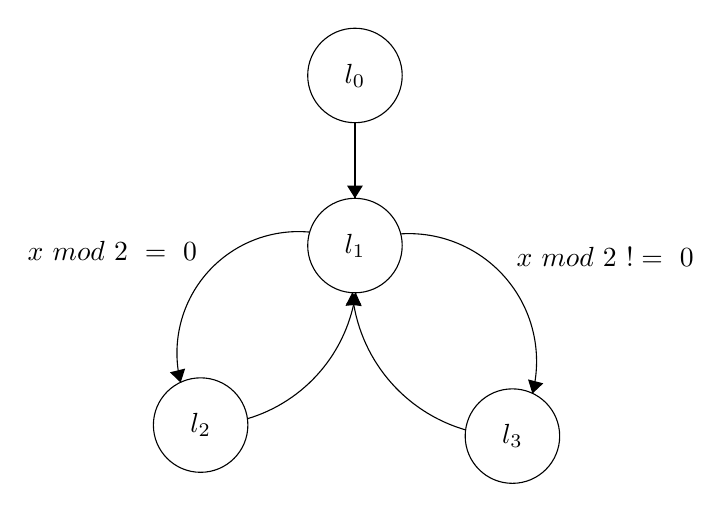
\begin{tikzpicture}[scale=0.2]
\tikzstyle{every node}+=[inner sep=0pt]
\draw [black] (37.3,-8.4) circle (3);
\draw (37.3,-8.4) node {$l_0$};
\draw [black] (37.3,-19.2) circle (3);
\draw (37.3,-19.2) node {$l_1$};
\draw [black] (27.5,-30.6) circle (3);
\draw (27.5,-30.6) node {$l_2$};
\draw [black] (47.3,-31.3) circle (3);
\draw (47.3,-31.3) node {$l_3$};
\draw [black] (37.3,-11.4) -- (37.3,-16.2);
\fill [black] (37.3,-16.2) -- (37.8,-15.4) -- (36.8,-15.4);
\draw [black] (26.228,-27.904) arc (-165.8972:-275.47075:7.712);
\fill [black] (26.23,-27.9) -- (26.52,-27.01) -- (25.55,-27.25);
\draw (27.31,-19.55) node [left] {$x\mbox{ }mod\mbox{ }2\mbox{ }=\mbox{ }0$};
\draw [black] (40.19,-18.46) arc (93.76859:-14.62479:8.111);
\fill [black] (48.57,-28.6) -- (49.26,-27.95) -- (48.29,-27.7);
\draw (47.53,-19.95) node [right] {$x\mbox{ }mod\mbox{ }2\mbox{ }!=\mbox{ }0$};
\draw [black] (37.349,-22.188) arc (-7.88184:-73.48611:9.751);
\fill [black] (37.35,-22.19) -- (36.74,-22.91) -- (37.73,-23.05);
\draw [black] (44.337,-30.909) arc (-106.08409:-174.77211:10.032);
\fill [black] (37.13,-22.18) -- (36.7,-23.03) -- (37.7,-22.93);
\end{tikzpicture}
\end{center}


\noindent Formalize this: $\texttt{Loc}: \{l_0,l_1,...\}, \texttt{Var}: \{x,pc\}, 
S: \texttt{Var} \rightarrow \texttt{Val} (\{x\} \rightarrow Z)$ and $\{\texttt{pc}\} \rightarrow \texttt{Loc}$. 
Now think about what the meaning of each edge is. Let $-->$ be a \texttt{State} $\times$ \texttt{State} \textit{successor} relation.


\begin{lstlisting}
   (l0,x:=e,l')           def
s-------------->s'        $\iff$      s(pc)=l $\wedge$ s'(pc) =l' $\wedge$ s'(x) = $[[e]]_s$

    (l,g,l')              def
s--------------> s'       $\iff$      s(pc) = l $\wedge$ s'(pc) = l' $\wedge$ $[[g]]_s$=true

\end{lstlisting}

\noindent Now that the meaning of the edges has been formalized, there are many ways
to proceed in defining the meaning of the program. Depending on what to analyze,
we can make a semantics. So what is the meaning of a program? We could be
interested in the value it computes, the set of reachable states, or something else.
A trace semantics says that the meaning of a program is its trace (list of values that the variables
take over time). Let's focus on the set of \texttt{Reach} of reachable states.\\

\noindent Define $\texttt{Init} = \{s|s(pc)=l_0\}$. Define the \texttt{Post} operator as the lifting of the state transition relation
to a function on sets of states that gives the set of $1$-step successors of a state. $\texttt{Post}: 2^{state} -> 2^{state}$. 

$$\texttt{Post}(S) = \{s' \in \texttt{State} | \exists s \in S.s--->s'\}$$

\noindent $ \texttt{Post}(S_1 \cup S_2) = \texttt{Post}(S_1) \cup \texttt{Post}(S_2)$ distributes because of exists operator. Easy to prove.
From this it follows that \texttt{Post} is Monotone (in terms of the sizes of the sets). IMPORTANT: Let $F = \lambda S. \texttt{Init} \cup \texttt{Post}(S)$.
Then the set of reachable states is least fix point $(lfp)_\emptyset^\sqsubseteq[F]$ of the function $F$, with respect to some ordering $\sqsubseteq$
and starting from the element $\emptyset$. 

$$\texttt{Reach} = (lfp)_\emptyset^\sqsubseteq[\lambda S. \texttt{Init} \cup \texttt{Post}(S))$$


\noindent Why does the least fix point exist / why is it well defined? We are using some general results of fixed point theory / order theory.\\

\noindent \textbf{Definition}: a complete lattice $D$ is a set $D$ with an ordering $\sqsubseteq$, smallest element $\bottom$, largest element $\top$, 
join function $\sqcup$, meet function $\sqcap$, such that:
\begin{itemize}
    \item $\sqsubseteq$ is a partial order on $D$
    \item join $\sqcup: 2^D \rightarrow D$ is the least upper bound with respect to $\sqsubseteq$
    \item meet $\sqcap: 2^D \rightarrow D$ is the greatest lower bound with respect to $\sqsubseteq$
    \item $\bottom = \sqcap D$
    \item $\top = \sqcup D$
    \item least upper bound and greatest lower bound exist for any subset of $D$
    \item an incomplete lattice has join and meet only defined for finite subsets
    \item every powerset forms a complete lattice where the ordering $\sqsubseteq$ is subset inclusion $\subseteq$,
          join $\sqcup$ is union $\cup$, meet $\sqcap$ is intersection $\cap$, bottom $\bottom$ is the empty set $\emptyset$,
          and top $\top$ is the full set itself. 
\end{itemize}


\noindent The powerset of states forms a complete lattice. Tarski's fixed point theorems say that
any monotone function over a complete lattice has a least fixed point. Abstract interpretation is approximating the set of fixed points for a function over a complete lattice.\\

\noindent Let's convince ourselves that definition of \texttt{Reach} makes sense. 
Let's look at some of the iterates of the fixed point functional $F=\lambda S. \texttt{Init} \cup \texttt{Post}(S)$:
\begin{itemize}
    \item $F$ applied $0$ times to $\emptyset: F^0(\emptyset) = \emptyset$
    \item $F$ applied $1$ time $F^1(\emptyset) = \texttt{Init}$
    \item $F^2(\emptyset) = \texttt{Init} \cup \texttt{Post}(\texttt{Init})$
    \item $F^3(\emptyset) = \texttt{Init} \cup \texttt{Post}(\texttt{Init} \cup \texttt{Post}(\texttt{Init}))$
\end{itemize}

\noindent Because of $\texttt{Post}'s$ distribution over $\cup$, the last line is equal to
$\texttt{Init} \cup \texttt{Post}(\texttt{Init}) \cup \texttt{Post}^2(\texttt{Init}).$ This gives us that
$F^k(\emptyset) = \cup_{i=0}^k F^i(\emptyset)$. Let $k$ go to the limit, we compute all reachable states.
\texttt{Reach} is the least fixed point starting from $\emptyset$  with respect to $\subseteq$ of $F$, which is equal to  $\cup_{i=0}^{\infty} F^i(\emptyset)$\\

\noindent Kleene says that if $D$ is a complete lattice, $F: D \rightarrow D$ is a function over that lattice, and $F$ is continuous in the following sense $(\star)$,
then the least fixed point starting from $\bottom$ with respect to the ordering $\sqsubseteq$ of $F$ is equal to $\sqcup_{i=0}^\infty F^i(\bottom)$.\\

\noindent $(\star)$ The definition of continuity here has various formulations, but the following is sufficient. If we take ascending chains 
in the ordering $d_0 \sqsubseteq d_1 \sqsubseteq d_2 ...$ (a sequence of potentially infinite elements increasing, perhaps not strictly increasing),
and if $F$ is known to be monotone,
and if we apply $F(d_0) \sqsubseteq F(d_1) \sqsubseteq F(d_2) ... $,
then $F$ distributes in the least upper bound of the new sequence so that $\sqcup_{i=0}^\infty\{F(d_i)\} = F(\sqcup_{i=0}^\infty\{d_i\})$. Winskel book has a discussion of this.\\

\noindent The least fixed point starting from $\bottom$ with respect to $\sqsubseteq$ of $F$ is $\sqcup_{i=0}^\infty\{F^i(\bottom)\}$.
It is an exercise to prove that our $F = \lambda S. \texttt{Init} \cup \texttt{Post}(S)$ is continuous.\\

\noindent This is a concrete semantics because it gives us the meaning of the program. This is already an abstraction in a way because it is not the trace semantics.
But this is our initial semantics: the set of reachable states. This has less info than traces, which by the way are also abstract in some sense.\\

\noindent Question: are there any more semantics with more info than trace semantics. 
In our language we have deterministic behavior. But think of a non-deterministic program.
Think about Temporal logics. How certain points of execution relate to each other. View of semantics of program as a tree. Like a non-deterministic Turing machine.
You may want to know whether there exists a branch in the tree that satisfies some property. Temporal logics like CTL and CTL* let you 
define these sort of things, define some notion of trees. Trace semantics would be an abstraction of the non-deterministic tree semantics\\

\noindent To be addressed soon: how can we prove that one notion of semantics is a sound abstraction of another?\\

\noindent Our problem: the set \texttt{Reach} can't be computed in general because of undecidability.
So rather than calculating \texttt{Reach} precisely, we approximate!\\

\noindent Remember our example program above. Consider a set of \texttt{Bad} states defined by a set of program counters $\{l_3\}$ (the else statement). 
Verification problem: is $\texttt{Reach} \cap \texttt{Bad} = \emptyset$? We need an inductive invariant, 
which is a set \texttt{Inv} of states that satisfies:
\begin{itemize}
    \item $\texttt{Inv} \supset \texttt{Init}$
    \item $\texttt{Post}(\texttt{Inv}) \subseteq \texttt{Inv}$
    \item $\implies \texttt{Reach} \subseteq \texttt{Inv}$
\end{itemize}

\noindent Look at this definition and thedefinition of \texttt{Reach}. Then \texttt{Reach} is the smallest, most precise invariant of the program. 
The set of all states is an invariant of the program too, but it doesn't tell us anything. The smallest set is the most informative. 
Anything that has the two invariant properties is guaranteed to be a superset of \texttt{Reach}. 
If we can show that $\texttt{Inv} \cap \texttt{Bad} = \emptyset$ then it also holds for \texttt{Reach}.\\

\noindent We want a way to automatically compute invariants to show that \texttt{Bad} states are not reachable. 
Aside from verification, we may also use invariants for optimization.\\

\noindent We approximate \texttt{Reach}. We approximate fixed points. How do we formalize this? When you do this analysis of the program, 
you approximate things on a different lattice, so that when you compute over that new lattice, you have the search for $F's$ fixed-point terminate.

\noindent Rough idea: Rather than keep track of the value of $x$, we could keep track of its parity (whether it is even or odd). 
Then we don't have to keep updating its value. Instead, we reason about whether or not we ever transition from even-ness to odd-ness, etc...\\

\noindent Abstract interpretation gives a mechanical process for coming up with another lattice for which the fixed-point search finishes and 
that is sound for the analysis we want to perform.\\


\noindent $D^\#$ (D sharp):

\begin{center}
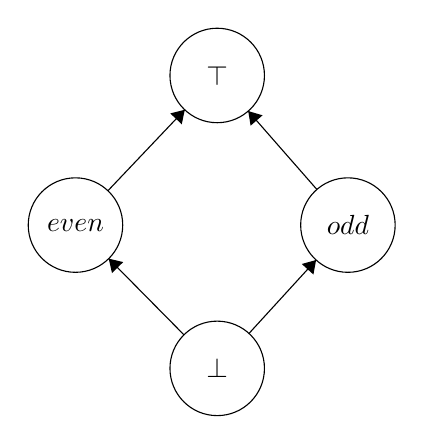
\begin{tikzpicture}[scale=0.2]
\tikzstyle{every node}+=[inner sep=0pt]
\draw [black] (36.2,-10.2) circle (3);
\draw (36.2,-10.2) node {$\top$};
\draw [black] (36.2,-28.8) circle (3);
\draw (36.2,-28.8) node {$\bottom$};
\draw [black] (27.2,-19.7) circle (3);
\draw (27.2,-19.7) node {$even$};
\draw [black] (44.5,-19.7) circle (3);
\draw (44.5,-19.7) node {$odd$};
\draw [black] (29.26,-17.52) -- (34.14,-12.38);
\fill [black] (34.14,-12.38) -- (33.22,-12.61) -- (33.95,-13.3);
\draw [black] (42.53,-17.44) -- (38.17,-12.46);
\fill [black] (38.17,-12.46) -- (38.32,-13.39) -- (39.08,-12.73);
\draw [black] (34.09,-26.67) -- (29.31,-21.83);
\fill [black] (29.31,-21.83) -- (29.52,-22.75) -- (30.23,-22.05);
\draw [black] (38.22,-26.58) -- (42.48,-21.92);
\fill [black] (42.48,-21.92) -- (41.57,-22.17) -- (42.31,-22.84);
\end{tikzpicture}
\end{center}


\noindent Even and Odd are incomparable, both larger than $\bottom$, both smaller than $\top$. 
How to relate this lattice to the original one? This lattice keeps track of the parity of $x$. 
We probably also want to keep track of the program counter. $D^\#$ is a lattice. 
The underlying set $\{\texttt{Loc} \rightarrow D^\#p\}$ is a set of functions. The lattice over-approximates values of $x$.\\

\noindent The ordering we choose on two functions holds if for all inputs, their results are ordered:
$s^\#_1 \sqsubseteq s^\#_2 \rightarrow \forall l \in \texttt{Loc}, s^\#_1(l) \sqsubseteq s^\#_2(l)$.
Aside: If $D$ is a complete lattice ordered by subset, then for all sets $X$, $X \rightarrow D$ 
is a complete lattice ordered by $\sqsubseteq$.\\

\noindent Galois Connections.\\

\noindent $\gamma$ (concretization): $D^\# \rightarrow 2^{State}$ is a mapping from our abstract lattice to our original concrete lattice.
\begin{align*}
    \gamma(\top) &= \texttt{State}\\
    \gamma(\bottom) &= \emptyset\\
    \gamma(\textrm{odd}) &= \{s \in \texttt{State}  | s(x) \texttt{ mod }2 \neq 0\}\\
    \gamma(\textrm{even}) &= \{s \in \texttt{State} | s(x) \texttt{ mod }2 = 0 \}
\end{align*}

\noindent We need $\gamma$ to exist and have a formal calculation, 
but we don't need to calculate it ever (what did this comment mean???)\\

\noindent To map concrete to abstract, we have $\alpha$ (abstraction): $2^Z \rightarrow D^\#_p$. Let's think about what we want for 
the relationship between $\gamma$ and $\alpha$. We want $Z \subset \gamma(\alpha(Z))$. If we do $a(Z) = T$, we lose too much info.
We can differentiate between whether the set to be mapped has all evens, all odds, or a mix.

\begin{align*}
    a(Z) = &|even, \textrm{ if } Z \subseteq \{z | z \texttt{ mod }2 = 0\}\\
           &|odd, \textrm{ if } Z \subseteq \{z | z \texttt{ mod }2 \neq 0\}\\
           &|\bottom, \textrm{ if } Z=\emptyset\\
           &|\top \textrm{ otherwise }
\end{align*}

\noindent Check the property we want, that $Z \subseteq \gamma(\alpha(Z))$.
Is it the best possible abstraction? We want $\alpha$ to have the tightest over-approximation for the given abstraction.
A Galois connection formalizes this idea. It's a pair of functions: $D \rightarrow^\alpha D\#$ and $D \leftarrow^\gamma D\#$
such that 
\begin{itemize}
    \item for all concrete values $x \in D$ and abstract values $y \in D\#$,  $\alpha(x) \sqsubseteq^\# y \iff  x \sqsubseteq \gamma(y)$
    \item $x \sqsubseteq \gamma(\alpha(x))$   [soundness] 
    \item $\alpha(\gamma(y)) \sqsubseteq^\# y$ [bestness]
    \item going to concrete and back to abstract can only give more information
\end{itemize}

\noindent With an abstraction in mind, we have a $\gamma$ and can we come up with an $\alpha$. 
When can you do this? You can do this when your gamma has certain properties.
$\gamma$ must be a complete $\sqcap$-morphism, which means that $\forall y \subseteq D\#$ (arbitrary subsets) 
$\gamma(\sqcap^\# y) = \sqcap( \{\gamma(y) | y \in Y \})$ and $\gamma(\top^\#)=\top$. 
If that's true, we can define $\alpha = \lambda x \in D . \sqcap\{y \in D\# | x \subseteq \gamma(y)\}$\\

\noindent Sometimes having $\alpha$ first is more natural. In that case you need to come up with a dual where you 
define a $\sqcup$-Morphism and construct $\gamma$, but normally you have a $\gamma$ in mind first and need to construct $\alpha$.
$\gamma(s\#) = \{s \in \texttt{State}| \forall l \in \texttt{Loc}. s(pc) = l \rightarrow s \in \gamma(s\#(l))\}$, which we can write as 
$\cup_{l \in \texttt{loc}} \{s \in \texttt{State}| s \in \gamma(s\#(l)) \wedge  s(pc) = l\}$.\\

\noindent Let's abstract $\texttt{Post}$. 
$\texttt{Post\#} : D\# \rightarrow D\#$. 
$\texttt{Post\#}(s\#) = \alpha(\texttt{Post}(\gamma(s\#)))$.
Composition of monotone functions is monotone. So the fixed point of \texttt{Post\#} exists on the abstract lattice.
$F\# = \lambda s\#. \texttt{Init\#} \cup \texttt{Post\#}(s\#)$. Let $p\#$ be the least fixed point of $F\#$ with respect to
$\sqsubseteq\#$ starting on $\bottom$. Then $\gamma(p\#) \supset \texttt{Reach}$.
$\texttt{Init}\#(l) = \top$ if $l=l_0$ and $\bottom$ otherwise.\\


\begin{lstlisting}
    $(l,x:=e,l')\#$
$s\#--------------> s'\#$   $\iff$ $s'\#(l')(x)=[[x]]^l_{s\#} \wedge $ (etc)
\end{lstlisting}


\noindent For the semantics of expressions like $[[e1+e2]]$, 
we can do $\alpha(\{z1+z2| z_1 \in \gamma([[e1]]^l_{s\#}) \wedge z_2 \in \gamma([[e2]]^l_{s'\#}) \})$. 
Abstract evaluation of expressions. Less precise than going from abstract state to concrete state, then evaluate whole expression in concrete, 
then back to abstract.\\

\noindent One way to keep track of a parity value of $x$ per location in the program is to do something like:
$(p_0 \textrm{ at } l_0, p_1 \textrm{ at }l_1, p_2 \textrm{ at }l_2, p_3 \textrm{ at }l_3)$. So our abstract function
$F\#$ maps abstract states to abstract states. $s_0\# -- (x:=(e=0))---> s_1\#  
\iff  (\bottom, p1', \bottom, \bottom)$ where $p_1' = [[e]]^{l_0}_{s_0\#}$ . 
Then $[[e=0]]$ gives us $(\bottom, even, \bottom, \bottom)$.\\

\noindent $\texttt{Post}\#$ is do \texttt{Post} for each transition, then take join of them. This is a function from $\texttt{Loc}$ to parity

\noindent Start from $\bottom$ and look at iterates of $F\#$:

\begin{align*}
\bottom\# =(def)= &(\bottom,\bottom,\bottom,\bottom)\\
F\#0(\bottom) = &(\bottom,\bottom,\bottom,\bottom)\\
F\#1(\bottom) = &(\top,\bottom,\bottom,\bottom)\\
F\#2(\bottom) = &(\top,even,\bottom,\bottom)\\ 
F\#3(\bottom) = &(\top,even,even,\bottom)\\
F\#4(\bottom) = &(\top,even,even,\bottom)
\end{align*}

\noindent So things left as bottom in the fixed point are unreachable, $l3$.\\

\noindent Consider x taking on intervals rather than even/odd. This corresponds to an infinite abstract domain.
The interval of $x$ will get larger as we iterate. How do we make sure the iterates converge so we find a fixed point?
The answer is the Widening operator:

\begin{itemize}
    \item $\nabla: D\# \times D\# \rightarrow  D\#$
    \item $\nabla$ approximates $\sqcup: y_1 \nabla y_2 \geq  y1,y2$
    \item sequence in abstract $y0 \sqsubseteq y1 \sqsubseteq ... $
    \item define $z0$ as $y0$, $z_i$ defined as  $z_{i-1} \nabla yi, i>0$
    \item $\rightarrow z0 \sqsubseteq z1 \sqsubset z2 ... $
    (also increasing due to upper bound property of $\nabla$ operator)
    must stabilize, so when we iterate we reach a fixed point.
\end{itemize}


\noindent Take the least fixed point starting on $\bottom$ with respect to $\sqsubseteq$ of $[\lambda y . y \nabla F\#(y)]$ 
for the old $F\#$ that we had. For each step, you widen with the previous iterate. How you define the widening operator is specific to the abstract domain.
Here you could do something simple, say, if $x$ increased then go right to $\infty$ for the right-side limit of the interval. 
Or perhaps wait a while (e.g. $x$ goes beyond $100$), and then go to $\infty$.
Choice of $\nabla$ is another layer of approximation! Though it seems that interval domain is more expressive than parity domain, it is sort of orthogonal.
We get information on whether $x$ takes on values in a range like [$0,\infty]$ (that is, $x$ is positive), but we don't know if its even or odd.\\

\noindent Galois connections compose



\end{document}




